\documentclass[
	% sans,			% use sans-serif font
	% serif,			% use serif-font
	%mathsans,		% set mathtext to sans-serif
	%mathserif,		% set mathtext to serif
	%10pt,
	10pt,
	%12pt,
	t		% add text at the top border of slide
	%slidescentered,% center text on slide
	%draft,			% compile as draft version
	%handout,		% create handout file
	%notes,			% include nodes in slides
	%compress		% compress navigation bar
]{beamer}

\usetheme{lmtslides}
\usepackage{eso-pic}
\usepackage{graphicx}
%\usepackage[pdftex]{color}
\usepackage{times}
\usepackage[latin1]{inputenc}
%\usepackage[T1]{fontenc}
\usepackage[amssymb]{SIunits}
\usepackage{amsmath,amssymb}
\usepackage{eurosym}
\usepackage{booktabs}
\usepackage{colortbl}
\usepackage{url}
\usepackage[absolute,overlay]{textpos}
\usepackage{graphicx}
\usepackage{mathtools}
\usepackage{pifont}% http://ctan.org/pkg/pifont
\usepackage{appendixnumberbeamer}
\usepackage{subcaption}
\usepackage{tikz}
\usepackage{pgfplots}


\usetikzlibrary{shapes.geometric, arrows}
\usetikzlibrary{positioning}
\usetikzlibrary{arrows}
\usetikzlibrary{calc}

\newcommand{\xmark}{\ding{55}}%
\newcommand{\cmark}{\ding{51}}%

\renewcommand{\footnoterule}{\vfill\kern -3pt  \kern 2.6pt}

\setbeamertemplate{caption}{\raggedright\insertcaption\par}
\setbeamertemplate{bibliography item}[online]
\graphicspath{{figures/}}

\setlang{en}		

% Supervisor: Univ.-Prof. Dr. Hans-Joachim Bungartz
% Advisors: Manish Kumar Mishra, M.Sc. (hons) &
% Samuel James Newcome, M.Sc.

% MODIFY THESE ACCORDINGLY! ---
\title{Algorithm Selection and Auto-Tuning in AutoPas}
\type{Sf} % (M/B/D/S)(f/m): (Master/Bachelor/Diplom/Studienarbeit)(final/midterm)
\author{Manuel Lerchner}
\email{manuel.lerchner@tum.de}
\advisorOne{Manish Kumar Mishra, M.Sc. (hons)}
\date{\today}
%------------------------------



\AtBeginSection[]
{
    \begin{frame}
        \frametitle{Table of Contents}
        \tableofcontents[currentsection,currentsubsection]
    \end{frame}
}

%%%%%%%%%%%%%%%%%%%%%%%%%%
\begin{document}

\maketitle

\setcounter{framenumber}{0}

\section{Introduction}

\begin{frame}{Molecular Dynamics Simulation Challenges}
    \begin{itemize}
        \item Complex interaction models
        \item Enormous numbers of particles
        \item High computational requirements
        \item Need for highly optimized algorithms
    \end{itemize}
\end{frame}

\begin{frame}{Traditional MD Engines vs AutoPas}
    \textbf{Traditional Engines (GROMACS, LAMMPS, ls1 mardyn):}
    \begin{itemize}
        \item Single, highly optimized implementation
        \item Static optimizations
        \item Hardware-specific tuning required
    \end{itemize}
    \vspace{0.5cm}
    \textbf{AutoPas Approach:}
    \begin{itemize}
        \item Dynamic optimizations
        \item Adapts to simulation state
        \item Hardware-independent
    \end{itemize}
\end{frame}

\section{AutoPas Framework}

\begin{frame}
    \frametitle{What is AutoPas?}

    \begin{textblock*}{5cm}(9cm,1.8cm)
        \includegraphics[width=3cm]{figures/AutoPasLogo}
    \end{textblock*}

    \begin{itemize}
        \item Library for arbitrary N-body simulations
        \item Optimal performance by switching implementations
              \begin{itemize}
                  \item \textbf{Container:} Finding neighboring particles
                  \item \textbf{Traversal:} Parallel force calculations
                  \item \textbf{Data Layout:} Memory access optimization
                  \item \textbf{Newton 3:} Force calculation optimization
              \end{itemize}
    \end{itemize}

    \vspace{-0.1cm}
    \begin{figure}
        \centering
        \includegraphics[width=0.72\textwidth]{figures/traversals.png}
    \end{figure}

    \begin{textblock*}{5cm}(6.3cm,9.35cm)
        \tiny{\cite{SIAM_PP24}}
    \end{textblock*}

\end{frame}


\begin{frame}
    \frametitle{Structure of AutoPas}

    \begin{itemize}
        \item Three main areas:
              \begin{itemize}
                  \item User Application
                  \item Algorithm Library
                  \item Tuning Strategies
              \end{itemize}
        \item Algorithm Library:
              \begin{itemize}
                  \item Huge Search Space\footnote{\scriptsize{$\text{Container}\times\text{Traversal} \times \text{Data Layout} \times \text{Newton 3} \times \text{Load Estimator} \times \text{Cell Size Factor}$}
                        }
              \end{itemize}
        \item Tuning Strategies:
              \begin{itemize}
                  \item Full Search
                  \item Random Search
                  \item Predictive Tuning
                  \item Bayesian Search
                  \item Rule Based Tuning
              \end{itemize}
    \end{itemize}

    \begin{textblock*}{4cm}(8cm,2cm)
        \begin{figure}
            \includegraphics[width=4cm]{figures/AutoPasLibraryStructure.png}
            \caption{ \scriptsize{\cite{Newcome2023Poster}}}

        \end{figure}
    \end{textblock*}
\end{frame}

\begin{frame}{Container Types}
    \begin{center}
        % \includegraphics[width=0.9\textwidth]{figures/containers.jpg}
    \end{center}
    \begin{itemize}
        \item Linked Cells
        \item Verlet Lists
        \item Verlet Cluster Lists
    \end{itemize}
\end{frame}

\begin{frame}{Traversal Patterns}
    \begin{center}
        % \includegraphics[width=0.9\textwidth]{figures/traversals.jpg}
    \end{center}
    \begin{itemize}
        \item C01: Independent cell processing
        \item C18: Color-based with Newton 3
        \item C08: Reduced synchronization points
    \end{itemize}
\end{frame}

\section{Auto-Tuning}

\begin{frame}{Tuning Strategies}
    \begin{itemize}
        \item \textbf{FullSearch:} Evaluates all configurations
        \item \textbf{RandomSearch:} Random sampling
        \item \textbf{BayesianSearch:} Optimization-guided selection
        \item \textbf{PredictiveTuning:} Performance prediction
        \item \textbf{RuleBasedTuning:} Expert knowledge rules
        \item \textbf{FuzzyTuning:} Fuzzy logic evaluation
    \end{itemize}
\end{frame}

\begin{frame}{Benefits of Auto-Tuning}
    \begin{itemize}
        \item Significant performance improvements
        \item Out-of-the-box optimization
        \item Hardware independence
        \item User-friendly interface
        \item Easy integration with other frameworks
    \end{itemize}
\end{frame}

\begin{frame}{Challenges of Auto-Tuning}
    \begin{itemize}
        \item Overhead from evaluating suboptimal configurations
        \item Unnecessary periodic re-tuning
        \item Complex scenarios needed to show benefits
    \end{itemize}
    \begin{center}
        \includegraphics[width=0.8\textwidth]{figures/unnecessary-tuning-phases.png}
    \end{center}
\end{frame}



\section{Early Stopping Optimization}


\begin{frame}{Early Stopping Idea}

    \begin{itemize}
        \item Each configuration gets evaluated multiple times
        \item Average performance is used for the final decision
        \item Optimization: Abort evaluation early if performance is poor
              \begin{itemize}
                  \item Stop after first poor sample
                  \item Stop during evaluation
              \end{itemize}
    \end{itemize}

    \vspace{0.8cm}

    \begin{center}
        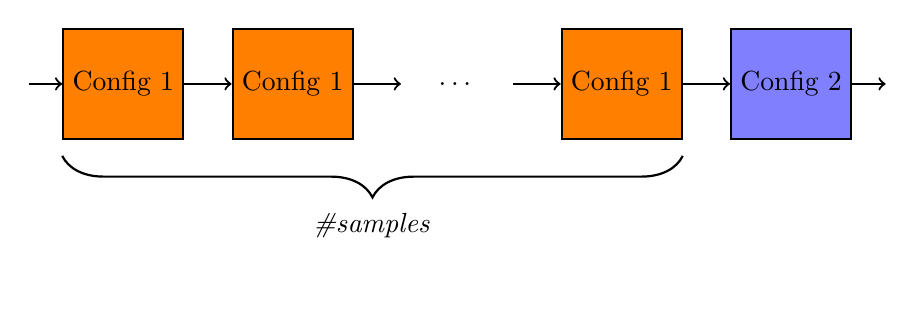
\begin{tikzpicture}[
                node distance=1.2cm and 0.6cm,
                every node/.style={draw, minimum width=1.4cm, minimum height=1.4cm, align=center},
                thick
            ]

            % Define nodes
            \node[fill=orange] (box1) {Config 1};
            \node[right=of box1,fill=orange] (box2) {Config 1};
            \node[right=of box2, style={draw=none}] (box3) {$\dots$};
            \node[right=of box3,fill=orange] (dots) {Config 1};
            \node[right=of dots,fill=blue!50] (boxN) {Config 2};

            % Arrows connecting boxes
            \draw[thick,<-] (box1) -- ++(-1.2,0);
            \draw[thick,->] (box1) -- (box2);
            \draw[thick,->] (box2) -- (box3);
            \draw[thick,->] (box3) -- (dots);
            \draw[thick,->] (dots) -- (boxN);
            \draw[thick,->] (boxN) -- ++(1.2,0);

            % Curly brace underneath the boxes
            \draw[decorate, decoration={brace, amplitude=15pt, mirror}, thick]
            ($(box1.south west) + (0,-0.2)$) -- ($(dots.south east) + (0,-0.2)$)
            node[midway, below=5pt,draw=none] {\textit{\#samples}};


        \end{tikzpicture}
    \end{center}
\end{frame}


\begin{frame}
    \frametitle{Implementation in AutoPas}

    \begin{itemize}
        \item Keep track of best performance seen so far
        \item Stop resampling if current performance exceeds optimal by a certain factor
        \item Hyperparameter: $allowedSlowdownFactor$

        \item Which $allowedSlowdownFactor$ should be used?
              \begin{itemize}
                  \item $allowedSlowdownFactor \rightarrow 1$: Many spurious aborts
                  \item $allowedSlowdownFactor \rightarrow \infty$: No early stopping
              \end{itemize}
    \end{itemize}
\end{frame}


\begin{frame}{Early Stopping Results [PredictiveTuning]}


    \begin{figure}[H]
        \centering

        \includegraphics[width=\columnwidth]{../../data/explodingLiquid/cluster/predictiveTuning/analytics/total_time_average.png}

        \caption{Total Simulation Time for Exploding Liquid Simulation for different values of $allowedSlowdownFactor$ using the PredictiveTuning strategy with early stopping.}
        \label{fig:predictive_tuning}
    \end{figure}


\end{frame}


\begin{frame}{Early Stopping Results Analysis}

    \begin{itemize}
        \item Reduction in total simulation time:
              \begin{itemize}
                  \item FullSearch: 14.8\% reduction
                  \item PredictiveTuning: 18.9\% reduction
              \end{itemize}
        \item Optimal threshold around 4.5
        \item Never significantly increased simulation time
    \end{itemize}
\end{frame}


\begin{frame}{Conclusion}
    \begin{itemize}
        \item AutoPas offers flexible, adaptive optimization
        \item Early stopping mechanism shows promise
        \item Trade-off between:
              \begin{itemize}
                  \item Specialized static optimization
                  \item Dynamic adaptability
              \end{itemize}
        \item Complementary approaches possible
    \end{itemize}
\end{frame}



\begin{frame}
    \begin{center}
        \vspace{1cm}
        {\large \textbf{Thank you for your attention!}}

        \vspace{2cm}

        \Huge{Questions?}
    \end{center}
\end{frame}




\begin{frame}[allowframebreaks, noframenumbering]
    \frametitle{References}
    \footnotesize
    \bibliographystyle{apalike}
    \bibliography{literature}
\end{frame}

\appendix

\begin{frame}
    \frametitle{Backup:}

    \begin{itemize}
        \item A
        \item B
    \end{itemize}
\end{frame}



\end{document}